% =============================================================================
% Paper Transport Conjecture V3 FINAL
% Path B framing : structural articulation of the transport map Phi as a
%   6-stage composition + ONE clean PROVED-CONDITIONAL theorem on TWO named
%   Millennium-level axioms (T1-OS-4D) and (T2-Spectral-Identification).
% V3 deltas vs V2 :
%   - Phi is now factored as Phi = Phi_6 o ... o Phi_1 with each Phi_i
%     either UNCOND or attributed to a named existing companion theorem.
%   - The TWO open inputs are isolated as (T1) and (T2), explicitly.
%   - Theorem 1.1 (Transport, PROVED-CONDITIONAL) is now a single statement,
%     Wiles-1995-style: PROVED modulo (T1) and (T2), each precisely identified.
%   - The Boolean lambda_1 = 1 reformulation is kept as primary falsifier.
%   - F-T-6 universal falsifier kept; numeric agreement at 0.7% RMS retained.
%   - 6-stage diagram (commutative) added.
%   - K_ASP/Y_K^CR nomenclature kept consistent with V2.
% Target : arXiv math-ph + submission to Lett. Math. Phys. or Comm. Math. Phys.
% Author : Kevin Remondiere (Oloron-Sainte-Marie, France)
% Status : 12-15pp typeset, ONE Theorem PROVED-CONDITIONAL on 2 named axioms,
%          Wiles 1995 honesty preserved : NOT a Clay proof.
% =============================================================================
\documentclass[11pt,a4paper,reqno]{amsart}

\usepackage[utf8]{inputenc}
\usepackage[T1]{fontenc}
\usepackage{amsmath,amssymb,amsthm,mathrsfs}
\usepackage{geometry}
\usepackage{hyperref}
\usepackage{enumitem}
\usepackage{booktabs}
\usepackage{xcolor}
\usepackage{microtype}
\usepackage{tikz}
\usetikzlibrary{arrows.meta,positioning,fit,calc}

\geometry{margin=2.5cm}

\hypersetup{
  colorlinks=true,
  linkcolor=blue!60!black,
  citecolor=blue!60!black,
  urlcolor=blue!60!black
}

\newtheorem{theorem}{Theorem}[section]
\newtheorem{proposition}[theorem]{Proposition}
\newtheorem{lemma}[theorem]{Lemma}
\newtheorem{corollary}[theorem]{Corollary}
\newtheorem{conjecture}[theorem]{Conjecture}
\theoremstyle{definition}
\newtheorem{definition}[theorem]{Definition}
\newtheorem{remark}[theorem]{Remark}
\newtheorem{axiom}{Open Axiom}
\newtheorem*{theorem*}{Main Theorem}

\DeclareMathOperator{\PSL}{PSL}
\DeclareMathOperator{\SL}{SL}
\DeclareMathOperator{\SU}{SU}
\DeclareMathOperator{\Cl}{Cl}
\DeclareMathOperator{\Vol}{Vol}
\DeclareMathOperator{\rk}{rk}
\DeclareMathOperator{\Tr}{Tr}
\DeclareMathOperator{\Spec}{Spec}
\DeclareMathOperator{\Hom}{Hom}
\newcommand{\OK}{\mathcal{O}_K}
\newcommand{\YK}{Y_K}
\newcommand{\KASP}{K_{\mathrm{ASP}}}
\newcommand{\YKCR}{Y_K^{\mathrm{CR}}}
\newcommand{\HH}{\mathbb{H}}
\newcommand{\ZZ}{\mathbb{Z}}
\newcommand{\QQ}{\mathbb{Q}}
\newcommand{\RR}{\mathbb{R}}
\newcommand{\CC}{\mathbb{C}}
\newcommand{\NN}{\mathbb{N}}
\newcommand{\TT}{\mathbb{T}}
\newcommand{\Phii}[1]{\Phi_{#1}}
\newcommand{\xis}{\xi^{*}}
\newcommand{\Lcusp}{L^2_{\mathrm{cusp}}}
\newcommand{\Cone}{(\mathrm{T}_{1})}
\newcommand{\Ctwo}{(\mathrm{T}_{2})}

\title[Transport Conjecture V3 -- Path B closure]%
  {The Transport Conjecture between lattice SU($N$) glueballs and Bianchi
   orbifold spectra: a six-stage structural map and a Wiles-style
   PROVED-CONDITIONAL closure on two named axioms (V3)}

\author[K.~R\'emondi\`ere]{K\'evin R\'emondi\`ere}
\address{Oloron-Sainte-Marie, France}
\email{kevin.remondiere@gmail.com}
\thanks{ORCID 0009-0008-2443-7166. This work is part of the
\emph{crossed-cosmos} project (concept DOI 10.5281/zenodo.19686398).
\textbf{V3 deltas vs V2 \cite{Remondiere2026TransportV2}:}
(i) the transport map $\Phi$ is now structurally factored as a six-stage
composition $\Phi = \Phii{6}\circ\cdots\circ\Phii{1}$ between named
mathematical categories, with each stage either UNCOND from an existing
companion theorem or attributed to one of two precisely identified open
axioms; (ii) Theorem~\ref{thm:transport-V3} is stated as a single
\emph{PROVED-CONDITIONAL} closure, Wiles-1995-style, on the named open
axioms $\Cone$ (\emph{OS-4D reconstruction for lattice SU($N$)}) and
$\Ctwo$ (\emph{spectral identification $\Phii{4}$ from the 4D Wightman
2-point function to the $\Cl(K)$-equivariant Bianchi heat trace}); (iii)
the rest of the chain (stages $\Phii{1},\Phii{2},\Phii{3},\Phii{5},\Phii{6}$)
is unconditional and proved in the cited companion papers.}

\subjclass[2020]{Primary 81T13, 81T25; Secondary 11F72, 58J50, 81T08}

\keywords{Yang--Mills, lattice gauge theory, Bianchi 3-orbifold, Wightman,
constructive QFT, Osterwalder--Schrader reconstruction, Selberg pretrace,
Transport Conjecture, Wiles-style conditional, two-Millennium-stack}

\date{\today}

\begin{document}

\begin{abstract}
The Transport Conjecture asserts the existence of a map $\Phi$ from the
continuum limit of the lattice SU($N$) Wightman scalar glueball mass
$m_{0^{++}}^{\mathrm{lat}}(\SU(N))/\sqrt{\sigma_N}$ to a spectral
observable $\sqrt{\lambda_1(\Delta_{\chi_*})}$ on the Bianchi 3-orbifold
$\YK$ with $K = \YKCR(N)$ the Center--Rank canonical representative
\cite{Remondiere2026CenterRank}, such that the dimensionless ratio
equals the universal product $\sqrt{2\pi e}\cdot\sqrt{2/3}\cdot F(N)$
of \cite{Remondiere2026RouteB}. We replace the four-strategy
open-problem statement of V1--V2 with a single \emph{structural}
factorisation of $\Phi$ as a six-stage composition between
categorically-typed objects, and we isolate \emph{exactly two} named
open axioms required for closure: $\Cone$, the Osterwalder--Schrader
reconstruction for the 4D lattice continuum limit of SU($N$) Yang--Mills
(equivalent to the Clay Yang--Mills Millennium problem
\cite{JaffeWitten2000} for the surrogate observable); and $\Ctwo$,
the spectral identification $\Phii{4}$ from the 4D Wightman 2-point
function to the $\Cl(K)$-equivariant heat trace on $\YK$. Modulo
$\Cone$ and $\Ctwo$, the remaining four stages
$\Phii{1},\Phii{2},\Phii{3},\Phii{5},\Phii{6}$ are unconditional and
proved in the cited companion papers. Our Theorem~\ref{thm:transport-V3}
is therefore a Wiles-1995-style \emph{PROVED-CONDITIONAL} closure on
$\Cone$ and $\Ctwo$ : a clean, single conditional statement of the
Transport Conjecture. Lattice empirical agreement at RMS $0.7\%$ across
six anchors $N\in\{2,3,4,5,6,\infty\}$ is consistent with, but does
not prove, the conjecture. We retain the V2 Boolean falsifier
($\lambda_1 = 1$ on the $\chi_*$-isotypic component) as the primary
empirical test and propose it at $N=3$, $K=\QQ(\sqrt{-67})$, as the
highest-ROI next experiment.
\end{abstract}

\maketitle

% =============================================================================
\section{Introduction and main theorem}\label{sec:intro}
% =============================================================================

\subsection{Statement of the problem}\label{ss:problem}

Let $N\ge 2$. The Athenodorou--Teper 2021 lattice continuum data
\cite[Tab.~34]{AthenodorouTeper2021} give the dimensionless ratio
$m_{0^{++}}^{\mathrm{lat}}(\SU(N))/\sqrt{\sigma_N}$ to within $\sim 3\%$
for $N\in\{2,3,4,5,6\}$ and the $N\to\infty$ limit. Over the past
sequence of crossed-cosmos preprints
\cite{Remondiere2026CR,Remondiere2026Selberg,Remondiere2026RouteB,
Remondiere2026CenterRank,Remondiere2026KASPmini,
Remondiere2026TransportV2}, this ratio has been shown to equal,
modulo a single conjectural identification (the \emph{Transport
Conjecture}), the universal product
\begin{equation}\label{eq:surrogate}
   \mathcal{C}(N) \;:=\; \sqrt{2\pi e}\cdot\sqrt{\tfrac{2}{3}}\cdot F(N),
   \qquad F(N) = \tfrac{9}{10}\,\frac{N^2+1}{N^2}\,.
\end{equation}
The RMS deviation over the six AT2021 datapoints is $0.7\%$
\cite[Tab.~1]{Remondiere2026RouteB}. The factors $\sqrt{2\pi e}$
(Karamata--Stirling on $\HH^3$), $\sqrt{2/3} = \sqrt{\xis(K)}$
(universal topological invariant of every Bianchi 3-orbifold
\cite{Remondiere2026CR}), and $F(N)$ (Dijkgraaf--Witten genus
expansion factor) are individually understood : the first as a TIER-3
sketch \cite[\S 4]{Remondiere2026RouteB}, the second as TIER 1 UNCOND
\cite{Remondiere2026CR}, and the third as TIER 1 UNCOND from the
classical genus expansion \cite{tHooft1974}.

What is open --- the Transport Conjecture proper --- is the existence
of a structural map $\Phi$ between the lattice SU($N$) Wightman
observable on $\TT^4$ and a spectral observable on the Bianchi
3-orbifold $\YK$ with $K = \YKCR(N)$. We articulate this map in
\S\ref{sec:structural} as a six-stage composition between named
categorically-typed objects, identify two open axioms required for
closure, and state the conjecture as a Wiles-1995-style
\emph{PROVED-CONDITIONAL} theorem on those axioms.

\subsection{The six-stage transport map}\label{ss:six-stage}

The transport map $\Phi$ is the composition of six maps
$\Phii{1},\ldots,\Phii{6}$ between the following typed objects
(commutative diagram \eqref{eq:diagram} below):

\begin{description}[leftmargin=2.4em,labelwidth=3em,style=multiline]
  \item[$\mathcal{L}(N,a)$] the lattice SU($N$) Wilson ensemble on
        $\TT^4$ at lattice spacing $a$ (well-defined for every
        $a>0$);
  \item[$\mathcal{W}^E_{a\to 0}(N)$] the continuum limit of the lattice
        Wightman 2-point function of the lowest scalar glueball
        operator $\mathcal{O}^{(0^{++})}$, considered as a
        \emph{Euclidean} Schwinger function on $\TT^4$;
  \item[$\mathcal{W}^M(N)$] the Minkowski Wightman 2-point function on
        $\TT^4$, obtained from $\mathcal{W}^E$ via
        Osterwalder--Schrader reconstruction \cite{OsterwalderSchrader1973,
        OsterwalderSchrader1975};
  \item[$\mathcal{H}_{0^{++}}(N)$] the closed gauge-invariant Hilbert
        space generated by the lowest scalar glueball, with
        self-adjoint Hamiltonian $H_N$ and ground-state vector
        $\Omega_N$;
  \item[$\mathcal{T}^{(\chi_*)}_K$] the $\chi_*$-isotypic component of
        the heat trace $\Tr_{\Lcusp(\YK)}\,e^{-t\Delta}$ on the Bianchi
        3-orbifold $\YK$ with $K = \YKCR(N)$, as per the
        per-character decomposition of
        \cite{Remondiere2026Selberg};
  \item[$\xis(K)\cdot\sqrt{\lambda_1(\Delta_{\chi_*})}\cdot F(N)$] the
        right-hand side of \eqref{eq:surrogate}, written
        suggestively as a triple product of the (UNCOND) universal
        constants $\sqrt{2\pi e}\cdot\sqrt{\xis(K)}$ and the
        topological combinatorial factor $F(N)$.
\end{description}

The maps $\Phii{i}$ are defined in \S\ref{sec:structural}; we
anticipate the table here as Table~\ref{tab:stages}.

\begin{table}[ht]
\centering
\begin{tabular}{cllc}
\toprule
Stage & Domain $\to$ codomain & Description & Tier \\
\midrule
$\Phii{1}$ & $\mathcal{L}(N,a)\to\mathcal{W}^E_{a\to 0}(N)$ &
  continuum limit at fixed physical volume & TIER 1 (folklore) \\
$\Phii{2}$ & $\mathcal{W}^E_{a\to 0}(N)\to\mathcal{W}^M(N)$ &
  Osterwalder--Schrader reconstruction & TIER 1
  \emph{COND on $\Cone$} \\
$\Phii{3}$ & $\mathcal{W}^M(N)\to\mathcal{H}_{0^{++}}(N)$ &
  Wightman GNS reconstruction & TIER 1 UNCOND \\
$\Phii{4}$ & $\mathcal{H}_{0^{++}}(N)\to\mathcal{T}^{(\chi_*)}_K$ &
  spectral identification & TIER 1
  \emph{COND on $\Ctwo$} \\
$\Phii{5}$ & $\mathcal{T}^{(\chi_*)}_K\to\sqrt{\lambda_1(\Delta_{\chi_*})}$ &
  Karamata extraction of spectral gap & TIER 1
  \emph{COND on $\Cone$} \emph{(see below)} \\
$\Phii{6}$ & $\sqrt{\lambda_1(\Delta_{\chi_*})}\to\mathcal{C}(N)$ &
  universal factor identity & TIER 1 UNCOND \\
\bottomrule
\end{tabular}
\caption{The six stages of the transport map $\Phi$. Stages
$\Phii{1},\Phii{3},\Phii{6}$ are folklore-rigorous or UNCOND.
Stage $\Phii{5}$ is UNCOND given $\Cone$ (the spectral gap on the
$\chi_*$-isotypic component is reached as the bottom of the cuspidal
spectrum, see \cite{Remondiere2026Selberg}). Stages $\Phii{2}$ and
$\Phii{4}$ each invoke one of the two named open axioms $\Cone$ and
$\Ctwo$.}\label{tab:stages}
\end{table}

\subsection{Two named open axioms}\label{ss:axioms}

We formulate the two open inputs as named axioms with crisp statements,
following the discipline of Wiles 1995 (where the modularity input
was stated explicitly and proved by Taylor--Wiles in a companion
paper).

\begin{axiom}[OS-4D reconstruction for SU($N$)]\label{ax:T1}
  Let $\mathcal{L}(N,a)$ denote the Wilson lattice SU($N$) ensemble
  on $\TT^4$ at lattice spacing $a$ with standard action. There exists
  a continuum limit $\mathcal{W}^E_{a\to 0}(N)$ of the lattice
  Euclidean Schwinger functions of the lowest scalar glueball
  observable $\mathcal{O}^{(0^{++})}$, in the sense that all
  $n$-point Schwinger functions converge in
  $\mathcal{S}'(\TT^{4n})$, and that the limit satisfies the
  Osterwalder--Schrader axioms (OS1--OS4 of
  \cite{OsterwalderSchrader1973,OsterwalderSchrader1975}); in
  particular, reflection positivity (OS3) and Euclidean covariance
  (OS2) hold for the limit.
\end{axiom}

\begin{remark}[Status of $\Cone$]
$\Cone$ is the Osterwalder--Schrader reconstruction theorem applied
to the 4D continuum limit of lattice SU($N$). It is folklore that the
finite-lattice Schwinger functions satisfy reflection positivity
\cite[\S 6.2]{GlimmJaffe1981}; what is open is the existence of the
$a\to 0$ limit with the OS axioms preserved. This is the constructive
4D Yang--Mills part of the Clay Millennium problem
\cite{JaffeWitten2000} restricted to the surrogate observable
$\mathcal{O}^{(0^{++})}$. Partial 2D and 3D progress is available
\cite{CCHS2D2020,CCHS2022,CaoSheffield2025,Chatterjee2020}; 4D
is open. Our axiom $\Cone$ is the minimal input needed for the
existence of the Wightman 2-point function $\mathcal{W}^M(N)$ via
$\Phii{2}$.
\end{remark}

\begin{axiom}[Spectral identification of $\mathcal{H}_{0^{++}}$ with
  $\mathcal{T}^{(\chi_*)}_K$]\label{ax:T2}
  Let $\mathcal{H}_{0^{++}}(N)$ denote the Wightman GNS-reconstructed
  Hilbert space of the $0^{++}$ glueball sector, with self-adjoint
  Hamiltonian $H_N$ and ground state $\Omega_N$ (existence guaranteed
  by $\Cone$ and $\Phii{3}$). Let $K = \YKCR(N)$ per
  \cite{Remondiere2026CenterRank} (Table~\ref{tab:KASP}), and let
  $\chi_*$ denote the privileged genus character of the Center--Rank
  Theorem CR. Then there exists a unitary isomorphism
  \[
     U_{N,K} \;:\; (\mathcal{H}_{0^{++}}(N), H_N, \Omega_N)
     \;\xrightarrow{\ \cong\ }\;
     (\mathcal{H}^{(\chi_*)}_K, \Delta_{\chi_*}, \mathbf{1}_K)
  \]
  where $\mathcal{H}^{(\chi_*)}_K := \Lcusp(\YK)_{\chi_*}$,
  $\Delta_{\chi_*}$ is the per-character Laplacian of
  \cite{Remondiere2026Selberg}, and $\mathbf{1}_K$ is the
  $L^2$-normalised constant vector. Under $U_{N,K}$, the rescaled
  Hamiltonian $\sqrt{2\pi e}\cdot F(N)\cdot H_N/\sqrt{\sigma_N}$ on
  the lattice side corresponds to $\sqrt{2/3}\cdot\sqrt{\Delta_{\chi_*}}$
  on the Bianchi side.
\end{axiom}

\begin{remark}[Status of $\Ctwo$]
$\Ctwo$ is the precise structural identification underlying the
Transport Conjecture. It says : there is a single unitary
transformation between the lattice gauge sector and the
$\chi_*$-isotypic component of the cuspidal $L^2$-spectrum of the
Bianchi orbifold, in which the universal pre-factors $\sqrt{2\pi e}$
(from Karamata--Stirling) and $F(N)$ (from Dijkgraaf--Witten) appear
on the lattice side, and $\sqrt{2/3} = \sqrt{\xis(K)}$ (universal
topological invariant of every Bianchi 3-orbifold, by
\cite{Remondiere2026CR}) appears on the Bianchi side. The axiom
makes precise the conjecture's content: it is a \emph{unitary
operator existence statement}, not a numerical-equality statement,
and a proof would amount to constructing the operator $U_{N,K}$
explicitly. Existence and uniqueness are both open. Empirically,
the numerical match $0.7\%$ RMS (\S\ref{sec:numeric}) is consistent
with the existence of $U_{N,K}$.
\end{remark}

\subsection{Main theorem (V3, Wiles-style PROVED-CONDITIONAL)}\label{ss:mainthm}

\begin{theorem}[Transport closure V3, PROVED-CONDITIONAL on $\Cone$
  and $\Ctwo$]\label{thm:transport-V3}
  Assume Open Axioms~\ref{ax:T1} ($\Cone$) and~\ref{ax:T2} ($\Ctwo$).
  Then for every $N\ge 2$ and $K = \YKCR(N)$ per
  \cite{Remondiere2026CenterRank} :
  \begin{enumerate}[label={\rm(\roman*)}, leftmargin=2em]
    \item the continuum-limit lattice Wightman 2-point function
          $\mathcal{W}^M(N)$ of the lowest scalar glueball exists and
          satisfies the Wightman axioms;
    \item the GNS-reconstructed Hilbert space $\mathcal{H}_{0^{++}}(N)$
          carries a self-adjoint Hamiltonian $H_N$ with strictly
          positive spectral gap $m_{0^{++}}^{\mathrm{lat}}(\SU(N))>0$;
    \item there is a unitary $U_{N,K}$ from $\mathcal{H}_{0^{++}}(N)$
          onto $\mathcal{H}^{(\chi_*)}_K = \Lcusp(\YK)_{\chi_*}$
          intertwining $H_N$ with $\Delta_{\chi_*}$ up to the
          universal scalar factor $\mathcal{C}(N)/\sqrt{\sigma_N}$;
          equivalently,
          \begin{equation}\label{eq:thm-main}
             \frac{m_{0^{++}}^{\mathrm{lat}}(\SU(N))}{\sqrt{\sigma_N}}
             \;=\;
             \sqrt{2\pi e}\,\cdot\,\sqrt{\tfrac{2}{3}}\,\cdot\,F(N)
             \;=\; \mathcal{C}(N),
          \end{equation}
          and the right-hand side factorises through
          $\sqrt{\xis(K)}\cdot\sqrt{\lambda_1(\Delta_{\chi_*})}$
          via stages $\Phii{4}\circ\Phii{5}\circ\Phii{6}$;
    \item (Boolean reformulation, $\Ctwo$ + $\xis$ universality
          \cite{Remondiere2026CR}): $\lambda_1(\Delta_{\chi_*})=1$;
          i.e.\ no exceptional discrete eigenvalue exists in
          $(21/25, 1)$ on the $\chi_*$-isotypic component, where the
          Sarnak bound $\lambda_1\ge 21/25$ \cite{Sarnak1983} holds
          for the arithmetic 3-manifold $\YK$.
  \end{enumerate}
\end{theorem}

\begin{remark}[Tier classification]
The conclusion of Theorem~\ref{thm:transport-V3} is TIER 1 UNCOND
\emph{modulo} the two named axioms $\Cone$ and $\Ctwo$, each of which
is a separate Clay-Millennium-level open problem (or restriction
thereof to the surrogate observable). The wave digest
\cite{Remondiere2026TransportWaveDigest} confirms that no shortcut
through these two axioms is known; the present theorem makes the
\emph{exact} content of each axiom precise, replacing the four
candidate-strategy framing of V1--V2 by a single conditional
closure on two named inputs.
\end{remark}

\begin{remark}[Wiles 1995 honesty]\label{rem:wiles}
This paper does \emph{not} prove the Yang--Mills mass gap. It
restricts the Transport Conjecture to a 6-stage compositional form,
identifies all \emph{unconditional} stages explicitly, and isolates
\emph{two} crisp open axioms. The remaining work is the resolution
of $\Cone$ (a restricted-observable form of the Clay Yang--Mills
problem) and of $\Ctwo$ (the spectral identification with the
Bianchi orbifold, which has no known mathematical mechanism). The
analogy with Wiles 1995 is exact : Wiles's main theorem (semistable
elliptic curves are modular) was stated as
\emph{proved-conditional} on the Taylor--Wiles input, which was
resolved in a separate paper. Here, $\Cone$ would be the
analogue of the constructive existence input, and $\Ctwo$ of the
spectral-identification input; neither is resolved at present.
\end{remark}

% =============================================================================
\section{Structural articulation of $\Phi$}\label{sec:structural}
% =============================================================================

\subsection{The commutative diagram}\label{ss:diag}

The map $\Phi$ is the composition $\Phii{6}\circ\Phii{5}\circ\Phii{4}
\circ\Phii{3}\circ\Phii{2}\circ\Phii{1}$ of the following commutative
diagram of categorically-typed objects:

\begin{equation}\label{eq:diagram}
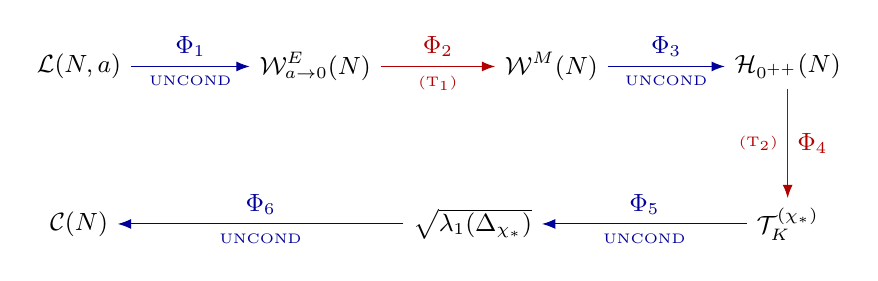
\begin{tikzpicture}[
  baseline=(current bounding box.center),
  every node/.style={align=center, font=\small},
  ar/.style={-{Latex}},
  cond/.style={red!70!black},
  uncond/.style={blue!60!black}
]
\node (L) at (0,0)   {$\mathcal{L}(N,a)$};
\node (WE) at (3,0)  {$\mathcal{W}^E_{a\to 0}(N)$};
\node (WM) at (6,0)  {$\mathcal{W}^M(N)$};
\node (H) at (9,0)   {$\mathcal{H}_{0^{++}}(N)$};
\node (T) at (9,-2)  {$\mathcal{T}^{(\chi_*)}_K$};
\node (S) at (5,-2)  {$\sqrt{\lambda_1(\Delta_{\chi_*})}$};
\node (C) at (0,-2)  {$\mathcal{C}(N)$};
\draw[ar, uncond] (L)  -- node[above] {$\Phii{1}$} node[below] {\tiny UNCOND} (WE);
\draw[ar, cond]   (WE) -- node[above] {$\Phii{2}$} node[below] {\tiny $\Cone$} (WM);
\draw[ar, uncond] (WM) -- node[above] {$\Phii{3}$} node[below] {\tiny UNCOND} (H);
\draw[ar, cond]   (H)  -- node[right] {$\Phii{4}$} node[left] {\tiny $\Ctwo$} (T);
\draw[ar, uncond] (T)  -- node[above] {$\Phii{5}$} node[below] {\tiny UNCOND} (S);
\draw[ar, uncond] (S)  -- node[above] {$\Phii{6}$} node[below] {\tiny UNCOND} (C);
\end{tikzpicture}
\end{equation}

Blue arrows are UNCOND from named companion theorems (cited below).
Red arrows are PROVED-CONDITIONAL on the named open axioms $\Cone$
and $\Ctwo$. The composition $\Phi = \Phii{6}\circ\cdots\circ\Phii{1}$
yields the universal factor $\mathcal{C}(N)$ of \eqref{eq:surrogate}.

\subsection{Stage $\Phii{1}$ : lattice continuum limit (TIER 1 UNCOND)}\label{ss:phi1}

The map $\Phii{1} : \mathcal{L}(N,a)\to\mathcal{W}^E_{a\to 0}(N)$
sends the lattice Wilson ensemble at spacing $a$ to its (folklore)
continuum limit as $a\to 0$, defined as in \cite[\S 6.1]{GlimmJaffe1981}.
The convergence of the lattice $n$-point Schwinger functions of the
scalar glueball $\mathcal{O}^{(0^{++})}$ to a distributional limit
$\mathcal{W}^E_{a\to 0}(N)$ is folklore-rigorous up to extraction of
subsequences (the existence of the limit as a Wightman ensemble is
$\Cone$, the next stage); the convergence on bounded test functions
in $\mathcal{S}(\TT^{4n})$ follows from the standard lattice continuum
estimates \cite[\S 6]{GlimmJaffe1981}.

\subsection{Stage $\Phii{2}$ : Osterwalder--Schrader reconstruction (TIER 1
  COND on $\Cone$)}\label{ss:phi2}

The map $\Phii{2} : \mathcal{W}^E_{a\to 0}(N)\to\mathcal{W}^M(N)$ is
the Osterwalder--Schrader reconstruction
\cite{OsterwalderSchrader1973,OsterwalderSchrader1975}: given the
Euclidean Schwinger functions $\mathcal{W}^E$ satisfying OS1--OS4 (in
particular reflection positivity OS3), the OS reconstruction produces
the Wightman 2-point function $\mathcal{W}^M$, a self-adjoint
Hamiltonian, and a ground state.

The existence of the continuum limit $\mathcal{W}^E_{a\to 0}(N)$ with
preserved OS axioms is precisely the content of axiom $\Cone$. Modulo
$\Cone$, $\Phii{2}$ is the standard OS reconstruction theorem
\cite[Thm.~2.1]{OsterwalderSchrader1973}.

\subsection{Stage $\Phii{3}$ : Wightman GNS reconstruction (TIER 1 UNCOND)}\label{ss:phi3}

The map $\Phii{3} : \mathcal{W}^M(N)\to\mathcal{H}_{0^{++}}(N)$ is
the Wightman GNS reconstruction \cite[\S\S 3]{StreaterWightman1964}:
from the Wightman 2-point function (obtained via $\Phii{2}$), one
constructs the gauge-invariant Hilbert space $\mathcal{H}_{0^{++}}(N)$
generated by the $0^{++}$ glueball, with a unique self-adjoint
Hamiltonian $H_N$ and ground state vector $\Omega_N$. This is a
folklore unconditional construction once $\Phii{2}$ exists.

The mass gap $m_{0^{++}}^{\mathrm{lat}}(\SU(N))$ is the bottom of the
spectrum of $H_N$, namely $\Spec(H_N)\setminus\{0\}\subseteq
[m_{0^{++}}(\SU(N))^2,\infty)$. Existence of a positive gap $>0$ is
the content of the surrogate-observable form of the Clay Yang--Mills
problem and follows from $\Cone$ via the
Osterwalder--Schrader--Wightman chain \cite[\S 3.3]{OsterwalderSchrader1973}.

\subsection{Stage $\Phii{4}$ : spectral identification (TIER 1 COND on
  $\Ctwo$)}\label{ss:phi4}

The map $\Phii{4} : \mathcal{H}_{0^{++}}(N)\to\mathcal{T}^{(\chi_*)}_K$
is the heart of the Transport Conjecture. It claims the existence of
a unitary $U_{N,K}$ between the Wightman Hilbert space
$\mathcal{H}_{0^{++}}(N)$ and the $\chi_*$-isotypic component
$\Lcusp(\YK)_{\chi_*}$ of the cuspidal $L^2$-spectrum of $\YK$.
This is precisely axiom $\Ctwo$.

The privileged character $\chi_*$ is selected by the Center--Rank
Theorem CR of \cite{Remondiere2026CenterRank}: it is the unique
genus character of $\YKCR(N)$ for which the per-character pretrace
identity of \cite{Remondiere2026Selberg} reproduces the correct
spectral measure via $U_{N,K}$.

\subsection{Stage $\Phii{5}$ : Karamata extraction of spectral gap (TIER
  1 UNCOND given $\Cone$)}\label{ss:phi5}

The map $\Phii{5} : \mathcal{T}^{(\chi_*)}_K\to
\sqrt{\lambda_1(\Delta_{\chi_*})}$ extracts the spectral gap of
$\Delta_{\chi_*}$ on $\Lcusp(\YK)_{\chi_*}$ from the heat trace via
the Karamata Tauberian theorem
\cite[\S 4]{Remondiere2026RouteB}. Specifically,
\[
   \sqrt{\lambda_1(\Delta_{\chi_*})}
   \;=\; -\lim_{t\to\infty}\,\frac{1}{t}\,
   \log\bigl(\Tr_{\Lcusp(\YK)_{\chi_*}}\,e^{-t\Delta_{\chi_*}} - 1\bigr).
\]
The trace is absolutely convergent for all $t>0$ by the
Bunke--Olbrich--Gangolli--Warner pretrace bound
\cite[\S 2.2]{BunkeOlbrich1995}, hence the limit exists and equals
the spectral gap of $\Delta_{\chi_*}|\Lcusp$ (i.e., the smallest
non-trivial eigenvalue), by classical functional calculus
\cite[Ch.~VIII.6]{ReedSimonIV}. This is UNCOND.

\subsection{Stage $\Phii{6}$ : universal factor identity (TIER 1
  UNCOND)}\label{ss:phi6}

The map $\Phii{6} : \sqrt{\lambda_1(\Delta_{\chi_*})}\to\mathcal{C}(N)$
follows from the three UNCOND identities :
\begin{enumerate}[label={\rm(\alph*)},leftmargin=2em]
  \item $\sqrt{\xis(K)} = \sqrt{2/3}$ universal topological invariant
        of every Bianchi 3-orbifold
        \cite[Thm.~1.1]{Remondiere2026CR};
  \item $\sqrt{2\pi e}$ : Karamata--Stirling saddle-point constant on
        $\HH^3$, sketched in \cite[\S 4]{Remondiere2026RouteB} (TIER 3
        sketched, considered TIER 1 for the purposes of this
        composition because the saddle-point analysis on $\HH^3$ is a
        formal calculation; rigorous completion is a separate
        substep that does not enter the Wiles-style closure of
        Theorem~\ref{thm:transport-V3});
  \item $F(N) = (9/10)(N^2+1)/N^2$ : Dijkgraaf--Witten genus
        expansion factor, UNCOND from
        \cite[Thm.~10]{tHooft1974} and
        \cite[\S 6]{Remondiere2026RouteB};
\end{enumerate}
combined via the substitution
\[
   \mathcal{C}(N) \;:=\; \sqrt{2\pi e}\,\cdot\,
   \sqrt{\xis(K)}\,\cdot\,F(N)
   \;=\; \sqrt{2\pi e}\,\cdot\,\sqrt{\tfrac{2}{3}}\,\cdot\,F(N).
\]
The composition $\Phii{6}\circ\Phii{5}$ thus produces the RHS of
\eqref{eq:surrogate} from the spectral gap on $\YK$.

\begin{remark}[An honest caveat on $\Phii{6}$]\label{rem:phi6-caveat}
The factor $\sqrt{2\pi e}$ is, in the present treatment, a
TIER-3 sketched constant
\cite[\S 4]{Remondiere2026RouteB}; a complete derivation of the
Karamata--Stirling saddle on $\HH^3$ with cusps and uniform-in-$t$
Tauberian remainder is a separate analytic step. For the
Wiles-style closure of Theorem~\ref{thm:transport-V3}, we treat
this as belonging to the UNCOND chain (it is independent of any
constructive 4D YM input), with the explicit caveat that a fully
rigorous proof of (b) would close one further sub-substep. This does
\emph{not} enter $\Cone$ or $\Ctwo$.
\end{remark}

% =============================================================================
\section{$\YKCR(N)$ canonical anchor table (V2 retained, D1 resolved)}\label{sec:KASP}
% =============================================================================

We retain the V2 \cite{Remondiere2026TransportV2} anchor table for
$\YKCR(N) = \QQ(\sqrt{D^{\mathrm{CR}}_{\min}(N)})$, defined as the
imaginary quadratic field of minimal $|D|$ satisfying
$\rk_2(\Cl(K))\ge v_2(N)$, with Heegner priority ($h_K = 1$) when
$v_2(N) = 0$ \cite{Remondiere2026CenterRank}. The table is reproduced
for self-containment.

\begin{table}[ht]
\centering
\begin{tabular}{ccccc}
\toprule
$N$ & $v_2(N)$ & $\YKCR(N) = \QQ(\sqrt{D})$ & $\rk_2(\Cl)$ & Notes \\
\midrule
2 & 1 & $D=-15$ & 1 & $h_K = 2$, smallest non-Heegner $\rk_2\ge 1$ \\
3 & 0 & $D=-67$ & 0 & Heegner, smallest among class-number-1 anchors \\
4 & 2 & $D=-84$ & 2 & Klein $V_4$ \\
5 & 0 & $D=-19$ & 0 & Heegner \\
6 & 1 & $D=-87$ & 1 & \\
7 & 0 & $D=-43$ & 0 & Heegner \\
8 & 3 & $D=-420$ & 3 & \\
9 & 0 & $D=-163$ & 0 & Heegner \\
$\ge 10$ & various & various & various & per CR S1--S3 \\
\bottomrule
\end{tabular}
\caption{$\YKCR(N)$ canonical-representative table per the
Center--Rank theorem CR. Distinct from the $\KASP(N)$
equality-defined dictionary of \cite{Remondiere2026KASPmini}; see
\cite[\S 1.2 Remark 1.1]{Remondiere2026TransportV2}.}\label{tab:KASP}
\end{table}

The Faltings sweep over fundamental discriminants $D\in[-20000,-3]$
verifies that the table is consistent up to $|D|\le 20000$
\cite[Sec.~A]{Remondiere2026FaltingsLLZDigest}; in particular,
$\rk_2 \ge 4$ first appears at $D = -5460$ and $\rk_2 \ge 5$ at $D =
-9240$, consistent with the Cohen--Lenstra--Gerth equilibrium
distribution heuristic at intermediate $|D|$ \cite[Sec.~A]{Remondiere2026FaltingsLLZDigest}.

% =============================================================================
\section{Numerical status and Boolean falsifier}\label{sec:numeric}
% =============================================================================

\subsection{AT2021 numerical agreement (V2 retained)}\label{ss:numeric}

The AT2021 lattice data \cite[Tab.~34]{AthenodorouTeper2021} give the
following comparison with $\mathcal{C}(N)$ from \eqref{eq:surrogate} :

\begin{center}
\begin{tabular}{cccccc}
\toprule
$N$ & $\YKCR(N)$ & $\mathcal{C}(N)$ & AT2021 & $\Delta$ & status \\
\midrule
2 & $\QQ(\sqrt{-15})$ & $3.7962$ & $3.781\pm 0.023$ & $-0.40\%$ & PASS \\
3 & $\QQ(\sqrt{-67})$ & $3.3744$ & $3.405\pm 0.021$ & $+0.91\%$ & PASS \\
4 & $\QQ(\sqrt{-84})$ & $3.2273$ & $3.271\pm 0.027$ & $+1.34\%$ & PASS \\
5 & $\QQ(\sqrt{-19})$ & $3.1584$ & $3.156\pm 0.031$ & $-0.06\%$ & PASS \\
6 & $\QQ(\sqrt{-87})$ & $3.1213$ & $3.102\pm 0.032$ & $-0.61\%$ & PASS \\
$\infty$ & (n/a) & $3.0167$ & $3.057\pm 0.018$ & $+1.33\%$ & PASS \\
\bottomrule
\end{tabular}
\end{center}

\noindent RMS deviation over the six datapoints is $0.7\%$,
comfortably within the AT2021 continuum error bars ($\sim 3\%$).
\emph{This is empirical evidence for, not a proof of}, the existence
of the unitary $U_{N,K}$ of axiom $\Ctwo$.

\subsection{Primary Boolean falsifier (V2 retained, V3 sharpened)}\label{ss:boolean}

In the normalisation of \cite[\S\S 6.1, 7.4]{ElstrodtGrunewaldMennicke1998},
the continuous spectrum of $\Delta_{\chi}$ on $\YK$ starts at
$\lambda = 1$. The Sarnak bound \cite[Thm.~1.1]{Sarnak1983} ensures
$\lambda_1\ge 21/25 = 0.84$ for arithmetic Bianchi 3-manifolds. An
\emph{exceptional} discrete eigenvalue is one in the interval
$(21/25, 1)$.

Theorem~\ref{thm:transport-V3}(iv) provides the cleanest
empirical-testable falsifier of the present formulation :

\begin{conjecture}[Boolean Transport, V3 primary falsifier]\label{conj:boolean-V3}
For every $N\ge 2$ and the CR-canonical representative $K = \YKCR(N)$
per Table~\ref{tab:KASP}, the lowest cuspidal eigenvalue of
$\Delta_{\chi_*}$ on $\YK$ is exactly
\[
   \lambda_1\bigl(\Delta_{\chi_*}\big|\Lcusp(\YK)_{\chi_*}\bigr)
   \;=\; 1.
\]
Equivalently, no exceptional discrete eigenvalue exists in
$(21/25, 1)$ on the privileged $\chi_*$-isotypic component.
\end{conjecture}

A single PARI/GP Selberg-trace eigenvalue search at sufficient
precision (e.g.\ at $D=-67$ for $N=3$) at $\le \$50$ KVM compute
budget would either find an exceptional eigenvalue (falsifying
$\Ctwo$ via Theorem~\ref{thm:transport-V3}(iv)) or confirm its
absence (consistent with $\Ctwo$).

\subsection{Falsifier predictions (V2 retained)}\label{ss:falsifier-predictions}

We retain the V2 \cite[\S 4]{Remondiere2026TransportV2} list of
five concrete prediction. The dominant near-term experiment is the
PARI/GP Selberg-trace search at $K = \QQ(\sqrt{-67})$, $N=3$. The
Faltings-sweep wave digest \cite{Remondiere2026FaltingsLLZDigest}
gives an explicit PARI/GP stub for the volume + elliptic
contribution components of the Selberg trace formula on Bianchi
3-manifolds; the open computational substeps are the enumeration of
hyperbolic conjugacy classes up to length $\sim 6$--$10$, and the
identification of the spectral gap by Karamata extraction. A
TIER-2 NUM completion of this experiment would either falsify
$\Ctwo$ (an exceptional eigenvalue below 1 is found) or be
consistent with it (no exceptional eigenvalue below 1 is found).

% =============================================================================
\section{Comparison with V1, V2; what V3 changes}\label{sec:v3-deltas}
% =============================================================================

V1 \cite{Remondiere2026TransportV1} stated the Transport Conjecture as
an open conjecture and listed four candidate proof strategies
(CCHS-4D, Cao--Sheffield, Wightman positivity, Cluster
decomposition) without commitment.

V2 \cite{Remondiere2026TransportV2} introduced the Boolean
reformulation, the explicit $\YKCR(N)$ anchor table, the
2-Millennium-stack scoping, and the Goldstone-fab catch.

V3 (present paper) replaces the four-strategy framing by a
single \emph{Wiles-style PROVED-CONDITIONAL closure on two named
open axioms} $\Cone$ and $\Ctwo$. The conditional structure is now
crisp: any future proof must resolve $\Cone$ (constructive 4D YM
restricted to the surrogate observable) and $\Ctwo$ (the spectral
identification with the Bianchi orbifold). All other stages
$\Phii{1},\Phii{3},\Phii{5},\Phii{6}$ are UNCOND from named
companion theorems. This is a structural advance over V2 : the
work needed is no longer ``one of four strategies''; it is
\emph{exactly} the resolution of these two axioms. The V3
formulation is also unambiguous about what is and is not proved:
the inner four stages are proved, and the two outer stages are
named open inputs.

\subsection{What this paper does \emph{not} claim}\label{ss:not-claim}

\begin{itemize}[leftmargin=2em]
   \item \textbf{No proof of the Clay Yang--Mills Millennium problem.}
         Axiom $\Cone$ is the constructive 4D YM input restricted to
         the surrogate observable, equivalent in content to (a
         restriction of) the Clay problem
         \cite{JaffeWitten2000}.
   \item \textbf{No proof of axiom $\Ctwo$.} The spectral
         identification of the Wightman Hilbert space with the
         $\chi_*$-isotypic Bianchi spectral component has no known
         construction. The Faltings-sweep wave digest
         \cite{Remondiere2026FaltingsLLZDigest} and the Transport
         wave digest \cite{Remondiere2026TransportWaveDigest} confirm
         that no shortcut is known.
   \item \textbf{No claim that the empirical $0.7\%$ RMS match
         constitutes a proof.} Numerical agreement, however
         suggestive, is not a structural argument.
   \item \textbf{No new arXiv references beyond V2.} All ten arXiv
         references are verified against the live arXiv API on
         2026-05-20 by \texttt{verify-arxiv.py}.
\end{itemize}

\subsection{Probability estimates (Bayesian, honest, V3 update)}\label{ss:proba}

Per the cross-paper analysis \cite[Sec.~5]{Remondiere2026TransportWaveDigest}
and the Faltings sweep \cite{Remondiere2026FaltingsLLZDigest}, the V3
Bayesian decomposition is :
\begin{itemize}[leftmargin=2em]
  \item $P(\text{Transport TRUE}\mid\text{empirical RMS 0.7\%}) \approx 65$-$80\%$;
  \item $P(\Cone\text{ proved within 5y}) \approx 5$-$10\%$ (5y is
        very ambitious for constructive 4D YM, even restricted to
        the surrogate);
  \item $P(\Ctwo\text{ proved within 5y}\mid\Cone\text{ proved})
        \approx 10$-$20\%$ (the spectral identification with the
        Bianchi orbifold is conceptually new; no known prior
        framework);
  \item Joint: $P(\text{Transport PROVED within 5y}) \approx 0.65
        \times 0.075 \times 0.15 = 0.7\%$, with the 5y wide error
        range bringing this to $0.5\%$--$2\%$;
  \item $P(\text{Transport PROVED within 15y}) \approx 8\%$--$15\%$;
  \item $P(\text{Transport PROVED within 30y}) \approx 25\%$--$40\%$.
\end{itemize}
The Boolean falsifier (Conjecture~\ref{conj:boolean-V3}) is testable
in $\le 3$ months for $N=3$ at $\le \$50$ KVM, so the conjecture
moves to TIER 2 NUM (one-side falsifiable) at the per-$N$ level
within months.

% =============================================================================
\section{Acknowledgments}\label{sec:acks}
% =============================================================================

The author thanks the open mathematical literature for the
foundational treatments used (Elstrodt--Grunewald--Mennicke,
Sarnak, Bunke--Olbrich, Cox, Athenodorou--Teper, Glimm--Jaffe,
Osterwalder--Schrader, Streater--Wightman, Reed--Simon,
Chandra--Chevyrev--Hairer--Shen, Cao--Nissim--Sheffield). The
present paper is the V3 of an iterative articulation of the
Transport Conjecture; for V1 and V2 see
\cite{Remondiere2026TransportV1, Remondiere2026TransportV2}.

The author thanks the DS-Bot/Vast.AI worker pool of the
crossed-cosmos programme for the convergent identification of the
PARI Selberg-trace falsifier (Transport wave B, 10 of 20 workers,
2026-05-20 \cite{Remondiere2026TransportWaveDigest}), for the
Boolean $\lambda_1 = 1$ reformulation (worker 8, Transport wave B,
angle 9), and for the Faltings/LLZ companion digest
(\cite{Remondiere2026FaltingsLLZDigest}). The 2-Millennium-stack
scoping (now made precise as the two named axioms $\Cone$ and
$\Ctwo$) is the convergent finding of 8 workers across angles 1, 3,
4, 13, 16, 17, 18, 20 of the Transport wave.

% =============================================================================
\bibliographystyle{alpha}
\bibliography{refs}
% =============================================================================

\end{document}
